\section[Traitement d'images]{Traitement d'images}

\begin{frame}{Application au traitement d'images}
	Dans cette section, on verra:
	\begin{itemize}
		\item Comment un algorithme d'apprentissage automatique traite des données de type images.
		\item Comment la méthode de l'analyse en composantes principales peut être utilisée pour simplifier un problème qui utiliserait des images en entrée.
	\end{itemize}
\end{frame}

\subsection[Représentation des images]{Représentation des images}

\begin{frame}{De l'image au vecteur (Aplatissement)}
	Pour comprendre comment un algorithme traite une image en \textbf{noir et blanc}, prenons un exemple simplifié : un \textbf{"0"} affiché sur une grille de $5 \times 3$ pixels.
	\begin{figure}
		\centering
		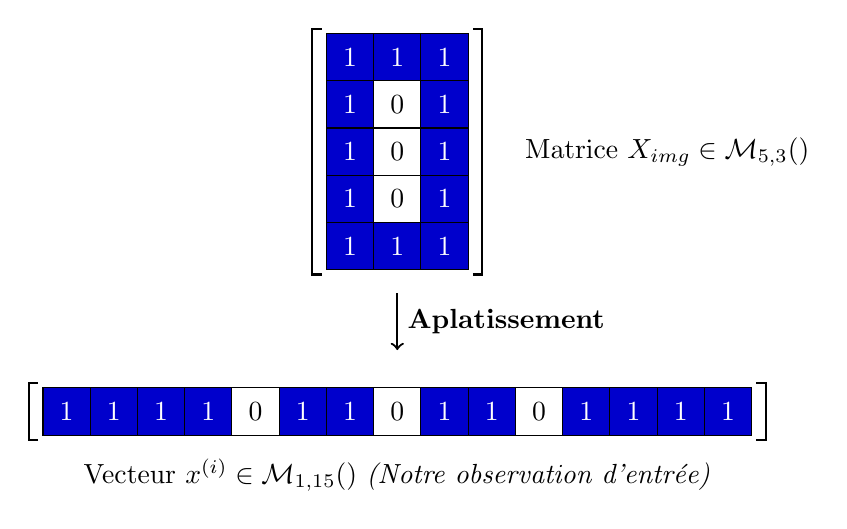
\begin{tikzpicture}[scale=0.6, every node/.style={minimum size=0.6cm}]
			% Définition des couleurs pour les pixels (bleu sombre pour 1, blanc pour 0)
			\colorlet{pixelon}{blue!80!black}
			\colorlet{pixeloff}{white}
			
			% --- MATRICE 5x3 (Centrée en haut) ---
			\begin{scope}[xshift=-1cm] 
				% Ligne 1
				\node[draw, fill=pixelon, text=white] at (0, 4) {1};
				\node[draw, fill=pixelon, text=white] at (1, 4) {1};
				\node[draw, fill=pixelon, text=white] at (2, 4) {1};
				% Ligne 2
				\node[draw, fill=pixelon, text=white] at (0, 3) {1};
				\node[draw, fill=pixeloff, text=black] at (1, 3) {0};
				\node[draw, fill=pixelon, text=white] at (2, 3) {1};
				% Ligne 3
				\node[draw, fill=pixelon, text=white] at (0, 2) {1};
				\node[draw, fill=pixeloff, text=black] at (1, 2) {0};
				\node[draw, fill=pixelon, text=white] at (2, 2) {1};
				% Ligne 4
				\node[draw, fill=pixelon, text=white] at (0, 1) {1};
				\node[draw, fill=pixeloff, text=black] at (1, 1) {0};
				\node[draw, fill=pixelon, text=white] at (2, 1) {1};
				% Ligne 5
				\node[draw, fill=pixelon, text=white] at (0, 0) {1};
				\node[draw, fill=pixelon, text=white] at (1, 0) {1};
				\node[draw, fill=pixelon, text=white] at (2, 0) {1};
				
				% Crochets de la matrice
				\draw[thick] (-0.6, -0.6) -- (-0.8, -0.6) -- (-0.8, 4.6) -- (-0.6, 4.6);
				\draw[thick] (2.6, -0.6) -- (2.8, -0.6) -- (2.8, 4.6) -- (2.6, 4.6);
			\end{scope}
			
			% Texte à côté de la matrice
			\node[right] at (2.5, 2) {Matrice $X_{img} \in \mathcal{M}_{5,3}(\R)$};
			
			% --- FLÈCHE D'APLATISSEMENT ---
			\draw[->, thick] (0, -1) -- (0, -2.2) node[midway, right] {\textbf{Aplatissement}};
			
			% --- VECTEUR 1x15 (Aplatissement ligne par ligne) ---
			\begin{scope}[xshift=-7cm, yshift=-3.5cm]
				% On dessine les 15 cases une par une pour un contrôle parfait
				\node[draw, fill=pixelon, text=white] at (0, 0) {1};
				\node[draw, fill=pixelon, text=white] at (1, 0) {1};
				\node[draw, fill=pixelon, text=white] at (2, 0) {1};
				
				\node[draw, fill=pixelon, text=white] at (3, 0) {1};
				\node[draw, fill=pixeloff, text=black] at (4, 0) {0};
				\node[draw, fill=pixelon, text=white] at (5, 0) {1};
				
				\node[draw, fill=pixelon, text=white] at (6, 0) {1};
				\node[draw, fill=pixeloff, text=black] at (7, 0) {0};
				\node[draw, fill=pixelon, text=white] at (8, 0) {1};
				
				\node[draw, fill=pixelon, text=white] at (9, 0) {1};
				\node[draw, fill=pixeloff, text=black] at (10, 0) {0};
				\node[draw, fill=pixelon, text=white] at (11, 0) {1};
				
				\node[draw, fill=pixelon, text=white] at (12, 0) {1};
				\node[draw, fill=pixelon, text=white] at (13, 0) {1};
				\node[draw, fill=pixelon, text=white] at (14, 0) {1};
				
				% Crochets du vecteur
				\draw[thick] (-0.6, -0.6) -- (-0.8, -0.6) -- (-0.8, 0.6) -- (-0.6, 0.6);
				\draw[thick] (14.6, -0.6) -- (14.8, -0.6) -- (14.8, 0.6) -- (14.6, 0.6);
				
				% Légende sous le vecteur
				\node[below] at (7, -0.8) {Vecteur $x^{(i)} \in \mathcal{M}_{1,15}(\R)$ \textit{(Notre observation d'entrée)}};
			\end{scope}
		\end{tikzpicture}
	\end{figure}
\end{frame}

\begin{frame}{De l'image au vecteur (Aplatissement)}
	Voici un autre exemple avec un \textbf{"4"}:
	\begin{figure}
		\centering
		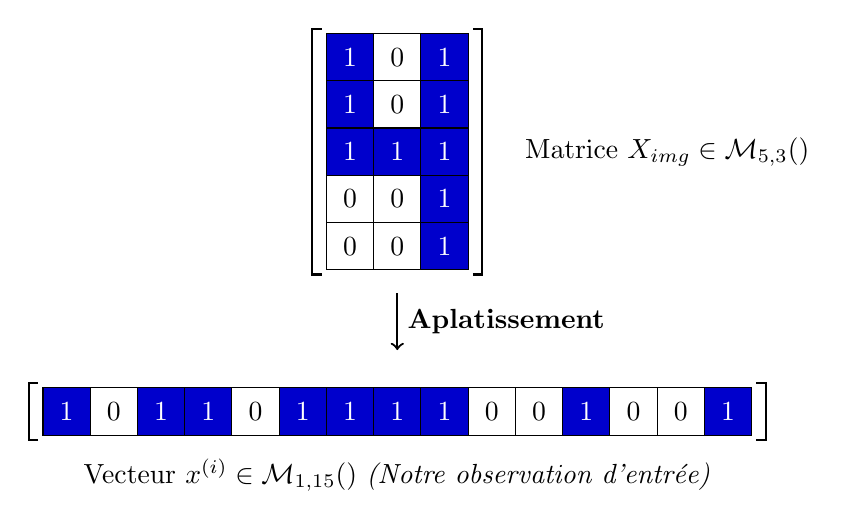
\begin{tikzpicture}[scale=0.6, every node/.style={minimum size=0.6cm}]
			% Définition des couleurs pour les pixels (bleu sombre pour 1, blanc pour 0)
			\colorlet{pixelon}{blue!80!black}
			\colorlet{pixeloff}{white}
			
			% --- MATRICE 5x3 (Centrée en haut) ---
			\begin{scope}[xshift=-1cm] 
				% Ligne 1
				\node[draw, fill=pixelon, text=white] at (0, 4) {1};
				\node[draw, fill=pixeloff, text=black] at (1, 4) {0};
				\node[draw, fill=pixelon, text=white] at (2, 4) {1};
				% Ligne 2
				\node[draw, fill=pixelon, text=white] at (0, 3) {1};
				\node[draw, fill=pixeloff, text=black] at (1, 3) {0};
				\node[draw, fill=pixelon, text=white] at (2, 3) {1};
				% Ligne 3
				\node[draw, fill=pixelon, text=white] at (0, 2) {1};
				\node[draw, fill=pixelon, text=white] at (1, 2) {1};
				\node[draw, fill=pixelon, text=white] at (2, 2) {1};
				% Ligne 4
				\node[draw, fill=pixeloff, text=black] at (0, 1) {0};
				\node[draw, fill=pixeloff, text=black] at (1, 1) {0};
				\node[draw, fill=pixelon, text=white] at (2, 1) {1};
				% Ligne 5
				\node[draw, fill=pixeloff, text=black] at (0, 0) {0};
				\node[draw, fill=pixeloff, text=black] at (1, 0) {0};
				\node[draw, fill=pixelon, text=white] at (2, 0) {1};
				
				% Crochets de la matrice
				\draw[thick] (-0.6, -0.6) -- (-0.8, -0.6) -- (-0.8, 4.6) -- (-0.6, 4.6);
				\draw[thick] (2.6, -0.6) -- (2.8, -0.6) -- (2.8, 4.6) -- (2.6, 4.6);
			\end{scope}
			
			% Texte à côté de la matrice
			\node[right] at (2.5, 2) {Matrice $X_{img} \in \mathcal{M}_{5,3}(\R)$};
			
			% --- FLÈCHE D'APLATISSEMENT ---
			\draw[->, thick] (0, -1) -- (0, -2.2) node[midway, right] {\textbf{Aplatissement}};
			
			% --- VECTEUR 1x15 (Aplatissement ligne par ligne) ---
			\begin{scope}[xshift=-7cm, yshift=-3.5cm]
				% On dessine les 15 cases une par une pour un contrôle parfait
				\node[draw, fill=pixelon, text=white] at (0, 0) {1};
				\node[draw, fill=pixeloff, text=black] at (1, 0) {0};
				\node[draw, fill=pixelon, text=white] at (2, 0) {1};
				
				\node[draw, fill=pixelon, text=white] at (3, 0) {1};
				\node[draw, fill=pixeloff, text=black] at (4, 0) {0};
				\node[draw, fill=pixelon, text=white] at (5, 0) {1};
				
				\node[draw, fill=pixelon, text=white] at (6, 0) {1};
				\node[draw, fill=pixelon, text=white] at (7, 0) {1};
				\node[draw, fill=pixelon, text=white] at (8, 0) {1};
				
				\node[draw, fill=pixeloff, text=black] at (9, 0) {0};
				\node[draw, fill=pixeloff, text=black] at (10, 0) {0};
				\node[draw, fill=pixelon, text=white] at (11, 0) {1};
				
				\node[draw, fill=pixeloff, text=black] at (12, 0) {0};
				\node[draw, fill=pixeloff, text=black] at (13, 0) {0};
				\node[draw, fill=pixelon, text=white] at (14, 0) {1};
				
				% Crochets du vecteur
				\draw[thick] (-0.6, -0.6) -- (-0.8, -0.6) -- (-0.8, 0.6) -- (-0.6, 0.6);
				\draw[thick] (14.6, -0.6) -- (14.8, -0.6) -- (14.8, 0.6) -- (14.6, 0.6);
				
				% Légende sous le vecteur
				\node[below] at (7, -0.8) {Vecteur $x^{(i)} \in \mathcal{M}_{1,15}(\R)$ \textit{(Notre observation d'entrée)}};
			\end{scope}
		\end{tikzpicture}
	\end{figure}
\end{frame}

\begin{frame}{Image en niveaux de gris}
	Une image dans une résolution 1280 x 720 pixels (dite résolution HD) en \textbf{niveaux de gris}:
	\begin{itemize}
		\item Est représentée dans un ordinateur par une matrice 720 par 1280. Quand on parle de résolution on parle en largeur x hauteur alors que la matrice associe la largeur aux colonnes et la hauteur aux lignes. C'est piégeur !
		\item Chaque élément de la matrice contient un entier entre 0 et 255 ($2^8$, soit 8 bits):
		\begin{itemize}
			\item 0: Le pixel sera noir.
			\item 255: Le pixel sera blanc.
			\item Les valeurs intermédiaires représentent des nuances de gris.
		\end{itemize}
		\item Pour les algorithmes d'apprentissage automatique on normalise les pixels afin que leur valeur soit entre 0 et 1.
		\item Une telle image représente donc une entrée de dimension 0,9 million: $720 \times 1280 = 921600$.
	\end{itemize}
\end{frame}

\begin{frame}{Image en couleurs}
	Une image dans une résolution 1280 x 720 pixels en \textbf{couleur}, dite RGB pour Red / Green / Blue:
	\begin{itemize}
		\item Est représentée dans un ordinateur par 3 matrices 720 par 1280, une pour chaque canal (rouge, vert ou bleu). On dit aussi \textbf{tenseur}, de dimension 720 x 1280 x 3.
		\item Chaque élément de la matrice contient un entier entre 0 et 255 ($2^8$, soit 8 bits):
		\begin{itemize}
			\item 0: Aucune intensité de la couleur courante, en fonction du canal.
			\item 255: Intensité maximale de la couleur courante.
			\item Les valeurs intermédiaires représentent des niveaux d'intensités de la couleur courante.
		\end{itemize}
		\item Pour les algorithmes d'apprentissage automatique on normalise les pixels afin que leur valeur soit entre 0 et 1.
		\item Une telle image est dite en 16 millions de couleurs: $256 \times 256 \times 256 = 16777216$
		\item Une telle image représente donc une entrée de dimension 2,7 millions: $720 \times 1280 \times 3 = 2764800$.
	\end{itemize}
\end{frame}

\begin{frame}{Exemples d'images}
	\begin{figure}
		\centering
		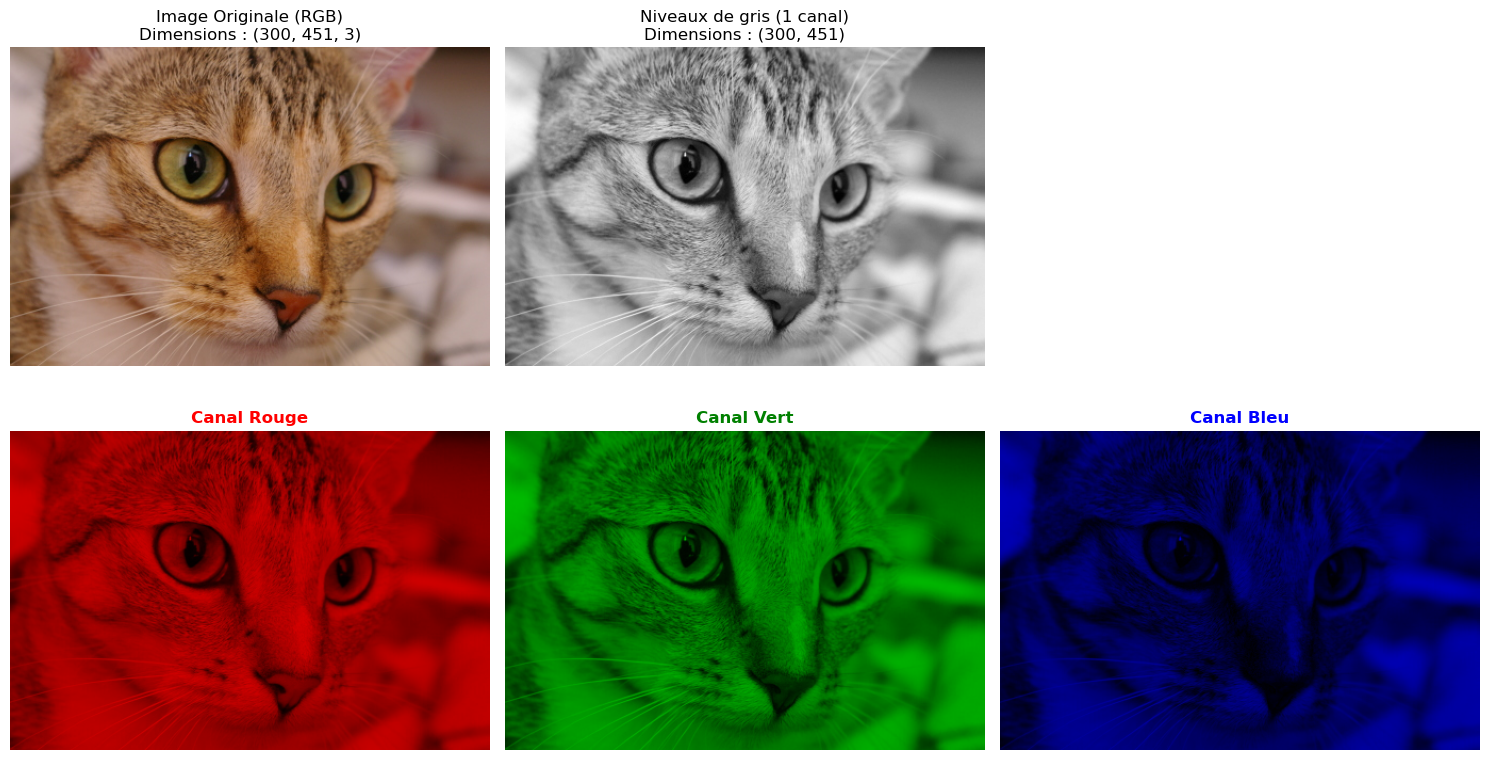
\includegraphics[width=1.0\linewidth]{Images/chelsea}
		\label{fig:chelsea}
	\end{figure}
\end{frame}

\begin{frame}{Exemples d'images}
	\begin{figure}
		\centering
		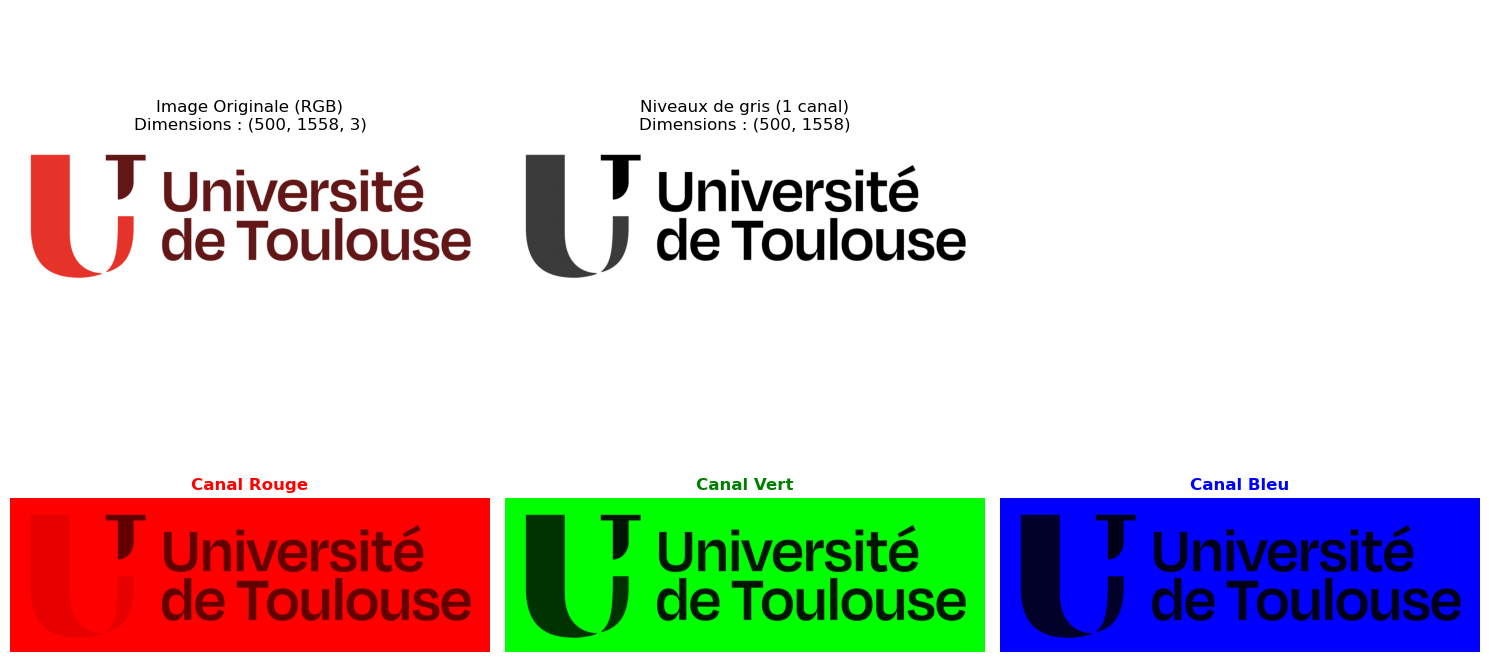
\includegraphics[width=1.0\linewidth]{Images/logo-UT-RGB}
		\label{fig:logo-UT-RGB}
	\end{figure}
\end{frame}

\subsection[ACP appliquée aux images]{ACP appliquée aux images}

\begin{frame}{Cas d'étude}
	Dans cette section, on appliquera l'analyse en composantes principales à des images. Comme nous l'avons vu précédemment, les images sont des entrées en très grandes dimensions. Toute simplification est alors bienvenue pour utiliser ces images en entrée d'un algorithme de régression ou de classification. \\
	\pause
	\vspace{0.5cm}
	On prendra pour exemple le dataset MNIST qui contient des images en niveaux de gris de chiffres écrits à la main: \href{https://www.kaggle.com/datasets/hojjatk/mnist-dataset}{\textbf{Kaggle MNIST Dataset}}.
	\begin{itemize}
		\item Yann LeCun, Courant Institute, NYU
		\item Corinna Cortes, Google Labs, New York
		\item Christopher J.C. Burges, Microsoft Research, Redmond
	\end{itemize}
\end{frame}

\begin{frame}{Exemples d'images}
	Les images disposent d'une résolution $28 \times 28 = 784$ et sont disponibles en niveaux de gris. Voici quelques exemples:
	\begin{columns}
		\begin{column}{0.33\textwidth}
			\begin{figure}
				\centering
				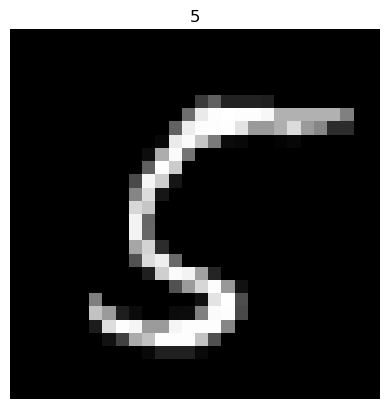
\includegraphics[width=1.0\linewidth]{Images/MNIST-5}
				\label{fig:MNIST-5}
			\end{figure}			
		\end{column}
		\begin{column}{0.33\textwidth}
			\begin{figure}
				\centering
				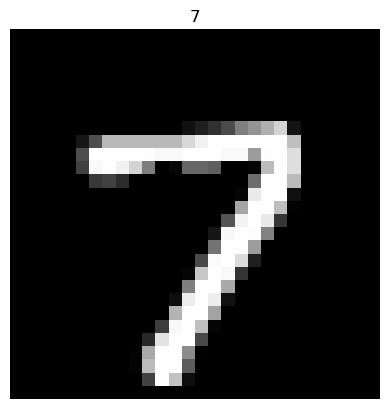
\includegraphics[width=1.0\linewidth]{Images/MNIST-7}
				\label{fig:MNIST-7}
			\end{figure}						
		\end{column}
		\begin{column}{0.33\textwidth}
			\begin{figure}
				\centering
				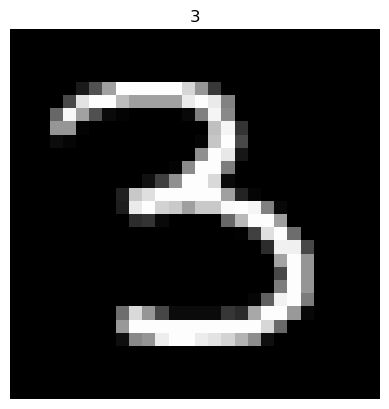
\includegraphics[width=1.0\linewidth]{Images/MNIST-3}
				\label{fig:MNIST-5}
			\end{figure}			
		\end{column}
	\end{columns}
\end{frame}

\begin{frame}{Traitement des images par ACP}
	Une image est donc un vecteur ligne de 784 valeurs ! Voici l'algorithme appliqué sur les images:
	\begin{enumerate}
		\item Tout d'abord on normalise les données. Comme chaque pixel peut valoir entre 0 et 255, on divise tous les termes par 255. Ce n'est pas obligatoire mais cela permet de conserver des valeurs propres relativement faibles.
		\item On centre les données en soustrayant l'image moyenne à chaque image.
		\item Exceptionnellement, on ne divise pas par la variance: un pixel qui se trouverait dans un coin de l'image a de fortes chances d'être noir et aurait donc une variance nulle. Comme tous les pixels ont des valeurs similaires, on s'en contentera, même si la variance de chaque pixel n'est pas unitaire.
		\item On calcule toutes les valeurs propres: \href{https://scikit-learn.org/stable/modules/generated/sklearn.decomposition.PCA.html}{\texttt{sklearn.decomposition.PCA}}.
		\item Cela nous permet de faire un tracé de l'éboulis des valeurs propres.
	\end{enumerate}
\end{frame}

\begin{frame}{\'Eboulis des valeurs propres du dataset MNIST}
	\begin{columns}
		\begin{column}{0.7\textwidth}
			\begin{figure}
				\centering
				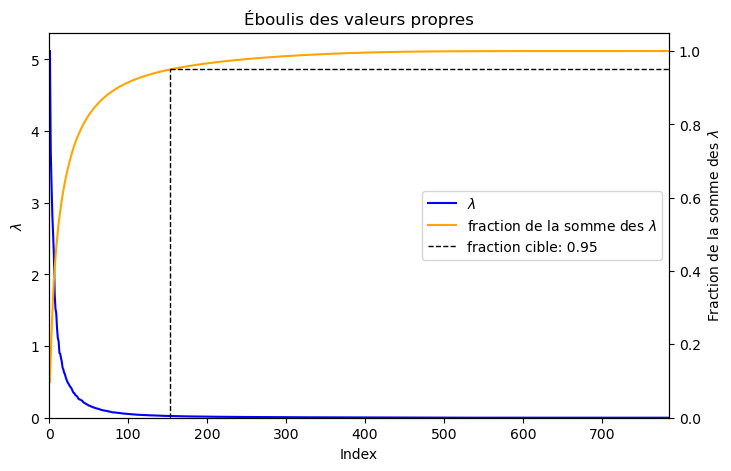
\includegraphics[width=1.0\linewidth]{Images/eboulis-MNIST}
				\label{fig:eboulis-MNIST}
			\end{figure}			
		\end{column}
		\begin{column}{0.3\textwidth}
			On peut conserver 95\% de la variance du dataset en ne conservant que les 150 plus grandes valeurs propres ! Cela permet de réduire la dimensionnalité du problème d'un facteur 5.
		\end{column}
	\end{columns}
\end{frame}

\begin{frame}{Conservation de toutes les composantes}
	En conservant l'intégralité des composantes, l'image reconstruite ($\hat{x}^{(i)}$) est parfaite. L'erreur $x^{(i)} - \hat{x}^{(i)}$ est nulle. Cela confirme bien que l'ACP redistribue la variance sans perte d'information:
	\begin{columns}
		\begin{column}{0.25\textwidth}
			\begin{figure}
				\centering
				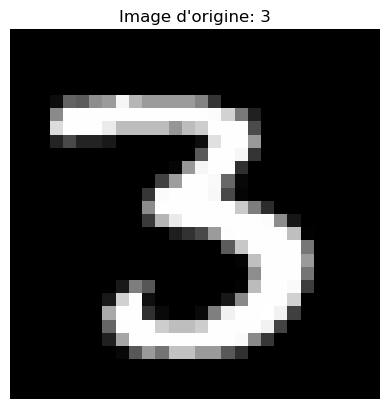
\includegraphics[width=1.0\linewidth]{Images/MNIST-3-28-origine}
				\label{fig:MNIST-3-28-origine}
			\end{figure}						
		\end{column}
		\begin{column}{0.25\textwidth}
			\begin{figure}
				\centering
				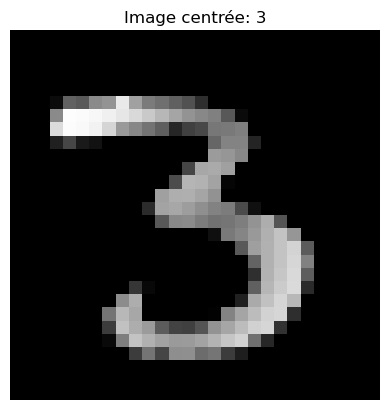
\includegraphics[width=1.0\linewidth]{Images/MNIST-3-28-centree}
				\label{fig:MNIST-3-28-centree}
			\end{figure}						
		\end{column}
		\begin{column}{0.25\textwidth}
			\begin{figure}
				\centering
				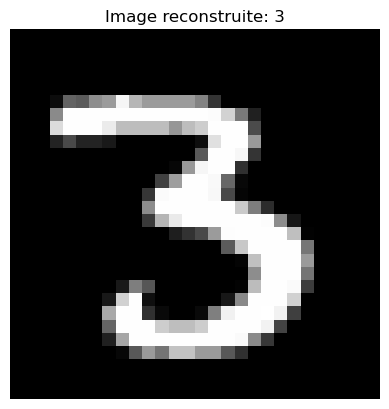
\includegraphics[width=1.0\linewidth]{Images/MNIST-3-28-reconstruite}
				\label{fig:MNIST-3-28-reconstruite}
			\end{figure}						
		\end{column}
		\begin{column}{0.25\textwidth}
			\begin{figure}
				\centering
				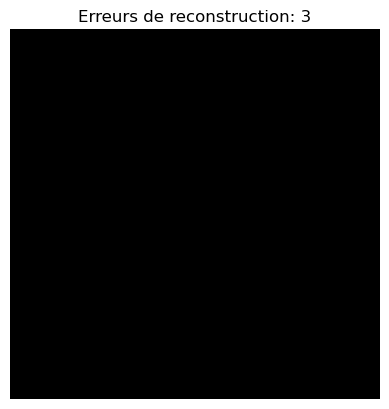
\includegraphics[width=1.0\linewidth]{Images/MNIST-3-28-erreur}
				\label{fig:MNIST-3-28-erreur}
			\end{figure}						
		\end{column}
	\end{columns}
\end{frame}

\begin{frame}{Conservation des 144 premières composantes}
	Notre tracé de l'éboulis de variance suggérait qu'avec environ 150 composantes conservées, 95\% de la variance était préservée. L'image reconstruite, sans être parfaite, est toujours reconnaissable facilement comme un \textbf{"3"}. L'erreur souligne un écart dans une zone très précise de l'image lors de la reconstruction:
	\begin{columns}
		\begin{column}{0.25\textwidth}
			\begin{figure}
				\centering
				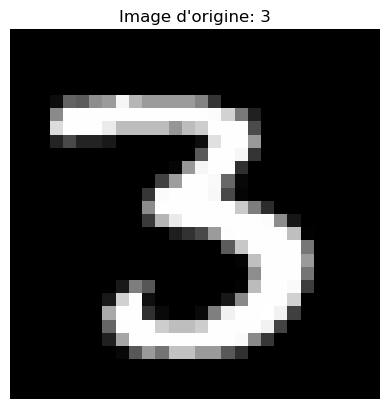
\includegraphics[width=1.0\linewidth]{Images/MNIST-3-12-origine}
				\label{fig:MNIST-3-12-origine}
			\end{figure}						
		\end{column}
		\begin{column}{0.25\textwidth}
			\begin{figure}
				\centering
				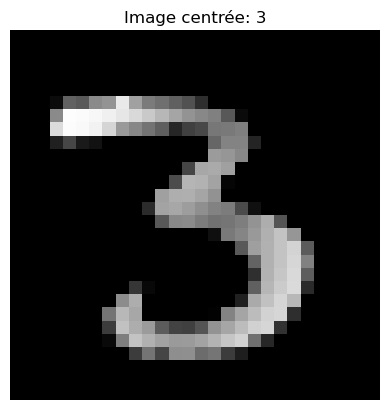
\includegraphics[width=1.0\linewidth]{Images/MNIST-3-12-centree}
				\label{fig:MNIST-3-12-centree}
			\end{figure}						
		\end{column}
		\begin{column}{0.25\textwidth}
			\begin{figure}
				\centering
				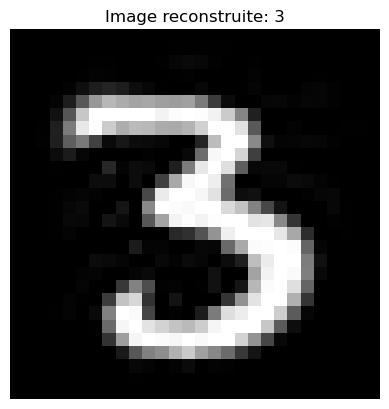
\includegraphics[width=1.0\linewidth]{Images/MNIST-3-12-reconstruite}
				\label{fig:MNIST-3-12-reconstruite}
			\end{figure}						
		\end{column}
		\begin{column}{0.25\textwidth}
			\begin{figure}
				\centering
				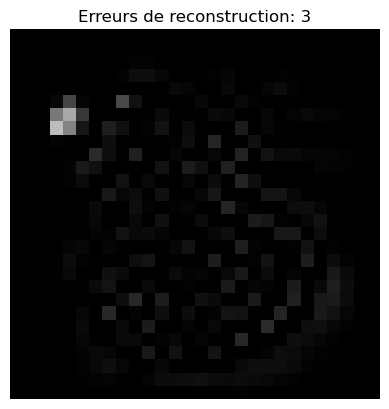
\includegraphics[width=1.0\linewidth]{Images/MNIST-3-12-erreur}
				\label{fig:MNIST-3-12-erreur}
			\end{figure}						
		\end{column}
	\end{columns}
\end{frame}

\begin{frame}{Conservation des 49 premières composantes}
	Réduire le nombre de composantes conservées à 49 commence à faire apparaître des erreurs importantes: on devine une forme de "3" dans l'erreur. L'image reconstruite reste lisible comme un "3" mais dispose maintenant d'une graphie très différente de l'image originale:
	\begin{columns}
		\begin{column}{0.25\textwidth}
			\begin{figure}
				\centering
				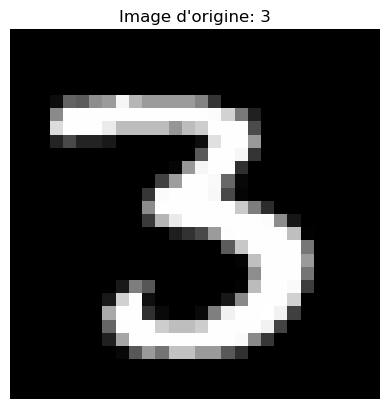
\includegraphics[width=1.0\linewidth]{Images/MNIST-3-7-origine}
				\label{fig:MNIST-3-7-origine}
			\end{figure}						
		\end{column}
		\begin{column}{0.25\textwidth}
			\begin{figure}
				\centering
				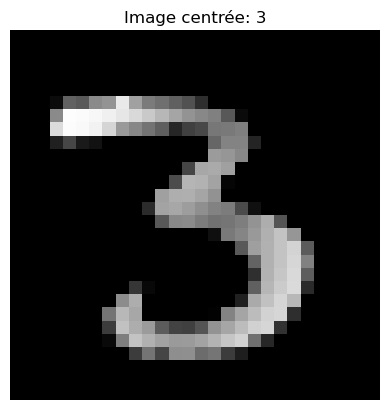
\includegraphics[width=1.0\linewidth]{Images/MNIST-3-7-centree}
				\label{fig:MNIST-3-7-centree}
			\end{figure}						
		\end{column}
		\begin{column}{0.25\textwidth}
			\begin{figure}
				\centering
				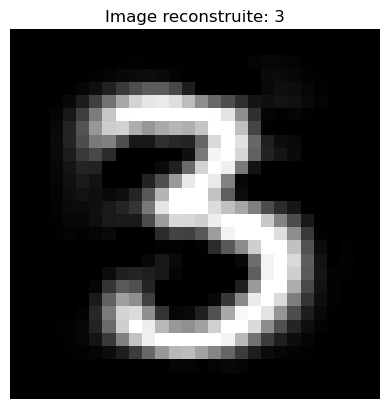
\includegraphics[width=1.0\linewidth]{Images/MNIST-3-7-reconstruite}
				\label{fig:MNIST-3-7-reconstruite}
			\end{figure}						
		\end{column}
		\begin{column}{0.25\textwidth}
			\begin{figure}
				\centering
				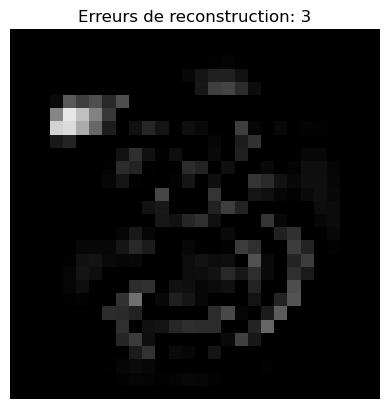
\includegraphics[width=1.0\linewidth]{Images/MNIST-3-7-erreur}
				\label{fig:MNIST-3-7-erreur}
			\end{figure}						
		\end{column}
	\end{columns}
\end{frame}

\begin{frame}{Conservation des 4 premières composantes}
	Dans ce cas extrême, seulement 4 composantes sont conservées. On distingue maintenant un "3" très visiblement sur les erreurs. L'image reconstruite ne ressemble plus vraiment à un "3". Trop d'information a été perdue en compressant aussi agressivement l'image:
	\begin{columns}
		\begin{column}{0.25\textwidth}
			\begin{figure}
				\centering
				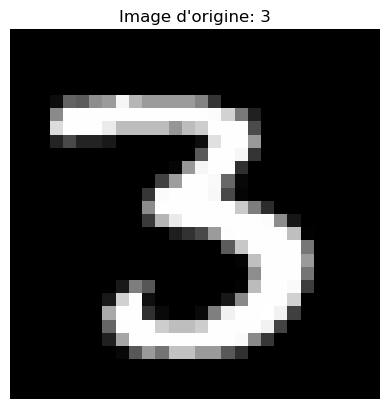
\includegraphics[width=1.0\linewidth]{Images/MNIST-3-2-origine}
				\label{fig:MNIST-3-2-origine}
			\end{figure}						
		\end{column}
		\begin{column}{0.25\textwidth}
			\begin{figure}
				\centering
				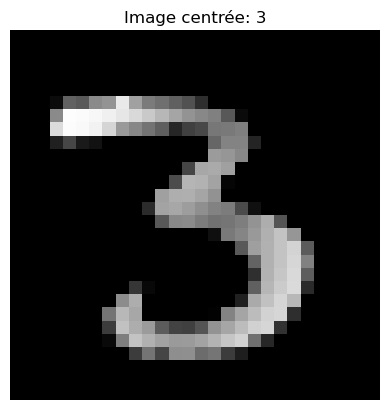
\includegraphics[width=1.0\linewidth]{Images/MNIST-3-2-centree}
				\label{fig:MNIST-3-2-centree}
			\end{figure}						
		\end{column}
		\begin{column}{0.25\textwidth}
			\begin{figure}
				\centering
				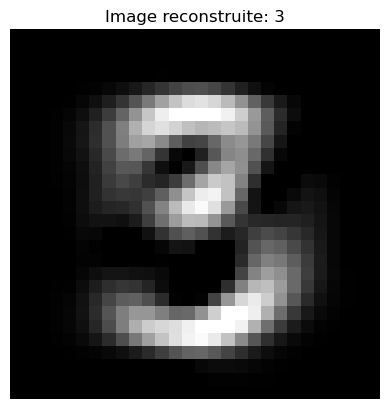
\includegraphics[width=1.0\linewidth]{Images/MNIST-3-2-reconstruite}
				\label{fig:MNIST-3-2-reconstruite}
			\end{figure}						
		\end{column}
		\begin{column}{0.25\textwidth}
			\begin{figure}
				\centering
				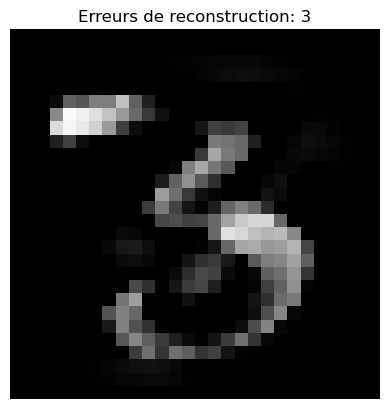
\includegraphics[width=1.0\linewidth]{Images/MNIST-3-2-erreur}
				\label{fig:MNIST-3-2-erreur}
			\end{figure}						
		\end{column}
	\end{columns}
\end{frame}